
\section{Proposed Methodology and Heuristics}
The first step will be to read in the words of the text under examination. The first naive approach will to just count the frequency of each word in a `bag of words' approach. This will be simple to implement initially, and won't require deep knowledge of natural language processing (NLP) algorithms that would be required to parse the sentence into a tree-like structure. Once the bag of words is constructed we can apply several proposed heuristics.

If the word frequency counting proves to not be powerful enough to capture the essence of the text, NLP algorithms such as those demonstrated by \cite{stanfordparser} will be researched in order to augment the approach. This would help to determine the meaning of a word, which in the english language is often determined by the context within a sentence.

\subsection{Odd Hyphenations}
A characteristic of puns that the authors have noticed is that they can sometimes contain `odd' hyphenations, or more precisely, hyphenations of words that are not commonly seen.

\begin{figure}[h]
\begin{mdframed}
  \emph{Atheism is a non-prophet organization.}
  \emph{A bicycle can't stand on its own because it is two-tired.}
  \caption{Puns with Odd Hyphenations}
 \label{oddhyphen}
\end{mdframed}
\end{figure}

In Figure~\ref{oddhyphen}, `non-prophet' (rather than `non-profit') and `two-tired' (rather than `too-tired') are hyphenations which most humans would deem as atypical. My idea would be to look for hyphenated phrases in a dictionary, or other datastore of figures of speech, and if the phrase isn't found, then we can perhaps make the assumption that it is a form of wordplay. 

\subsection{Homophones}
Puns often of homophones in them. A homophone is defined as being each of two or more words having the same pronunciation but different meanings, origins, or spelling, e.g., new and knew

\begin{figure}[h]
\begin{mdframed}
  \emph{What did the grape say when it got stepped on? Nothing - but it let out a little whine.}
  \caption{Pun with Homophones}
 \label{punhomophone}
\end{mdframed}
\end{figure}

In Figure~\ref{punhomophone}, the wordplay using homophones is `whine' which is a play on `wine' which is related to 'grape'. By looking for homophones of `whine', we would be led to `wine', which we could then make a linkage to grapes and winemaking, using a dictionary or encyclopedia.

\subsection{Dictionary Definitions}

\begin{figure}[h]
\begin{mdframed}
  \emph{I used to be addicted to soap, but I'm clean now.}
  \caption{Pun with terms linked by dictionary definitions}
 \label{addicted}
\end{mdframed}
\end{figure}

In Figure~\ref{addicted}, we can see some key words, `addicted', `clean' and `soap' have the connections between them that constitute a pun. For this example, we would process `addicted', and possibly find references to `clean', and the dictionary definition of `soap' could also have references to `clean'. When we see that `clean' has different definitions, with rather disparate meaning, we may be able to glean that there is a pun present.

\subsection{One letter mutations}

\begin{figure}[h]
\begin{mdframed}
  \emph{Did you see the movie about the hot dog? It was an Oscar Wiener.}
  \caption{Pun with relevant 1 letter mutation}
 \label{punmutation}
\end{mdframed}
\end{figure}

In Figure~\ref{punmutation} it can be seen that `Wiener'  is one letter removed from being the word `Winner', which is an appropriate reference to movies and the Oscar's awards show. By looking for other words which have a single letter different, it can help us to make linkages to the other parts of the sentence, using our other techniques. This could be efficiently computed using regular expressions, and a simple list of english words.

\subsection{Synthesized speech with dictionary search}
\begin{figure}[h]
\begin{mdframed}
  \emph{The roundest knight at king Arthur's round table was Sir Cumference.}
  \caption{Pun with audible word play}
 \label{sircumference}
\end{mdframed}
\end{figure}

In Figure~\ref{sircumference}, the word play of the phrase comes out when it is spoken. In this case, the Knight's name `Sir Cumference' becomes a homophone with `circumference'.
A stretch goal for this research could be to process text with text to speech software, and then back again from the generated audio, back into text. If the transformed text
differs from the input text, it could be indicative of audible word play. Of course this technique has its difficulties, and depends upon the quality of the text to speech, and speech to text synthesizers.

\section{A Reuseable Graph Data Structure}

An hypothesis that  we propose is that a graph data structure could be the best way for a computer program to catalogue and make use of connections between words in humorous text. As humans automatically maintain a mapping of incongruities, relationships, and connections between parts of a sentence, a graph could be constructed to represent the state of the analysis that a computer makes against a piece of text. 

The graph would have different types of nodes and edges, depending on what is being represented. For example, there would be a class of nodes that represent elements of the text under analysis, and there would also be nodes that represent `commonalities' between parts of the text. An example of a commonality could be a related subject between two words, such as `sports' between the elements `ball' and `score'. Another type of node could be 'parts of speech' information, which would allow different analytic modules to categorize parts of the sentence as verbs, adjectives, nouns, or as being part of a figure of speech. Adding this extra information could be required for more advanced humor detecting heuristics.

While in normal graphs, the edges don't necessarily carry much data of their own, the edges between nodes in this system are important because they define many different types of relationships between words. Some examples of different types of edges could be `homophone' edges denoting that two nodes are homophones of each other, or a 'figure of speech' edge which denotes that several nodes belong to another `figure of speech' node, denoting an idiomatic use of language. See Figure~\ref{pungraph} for an example of a Pun Graph that has been decorated by various heuristics.

\begin{center}
\begin{figure}[h]
  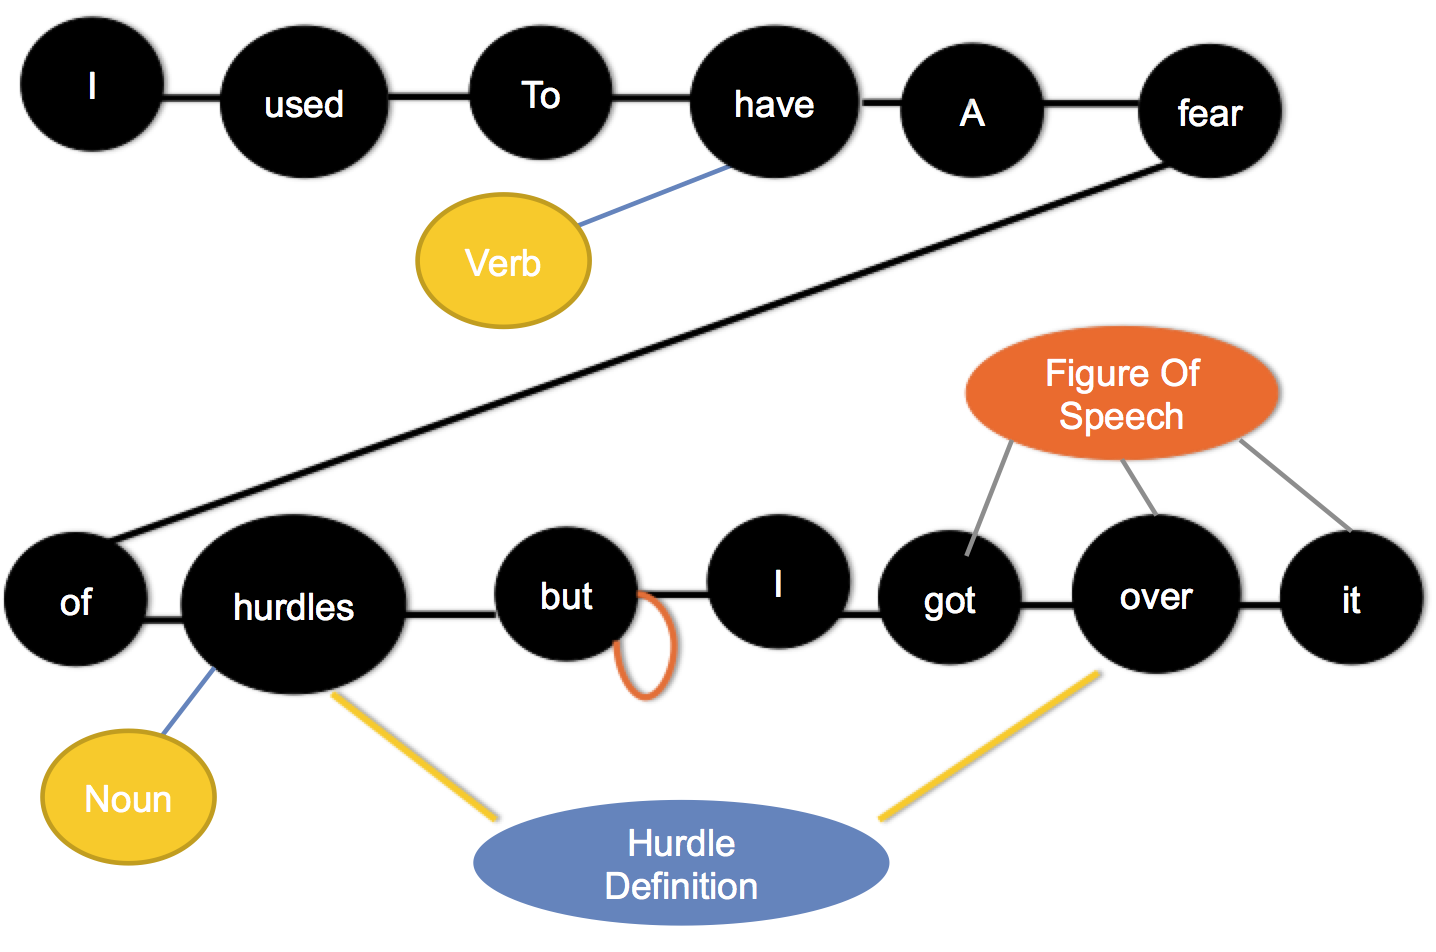
\includegraphics[keepaspectratio=true, scale=.35]{pun-graph-example.png}
  \caption{A Decorated Pun Graph}
   \label{pungraph}
\end{figure}
\end{center}

\subsection{Generalized scoring}
Because all edges and nodes inherit from the base classes that I will design, it makes the implementation of summing the contributions of all heuristics easy. To illustrate the general idea of how the system will use the graph, please refer to Algorithm~\ref{graphalgorithm}. The list of heuristics to be ran could potentially be a dynamically generated set, and the number of rounds of analysis could be bound by a timer or other upper limit, to ensure that the computation happens within a timely manner, or perhaps continues longer to become more rigorous.

\begin{algorithm}[h]
\begin{mdframed}
 \KwData{Input $text$}
 \KwData{Pun Graph $G$}
 \KwResult{Pun Score for the text, cumulatively assigned by all heuristics}
 Initialize graph $G$ with the Input $text$\;
 Initialize $score = 0$\;
 \While{there are heuristics left to run}{
      run heuristic on graph $G$\;
      update graph $G$ with additional nodes and edges\;
      next heuristic;
    }
  \For{$node \in G$}{
	 $score$ = $score$ + contribution of $node$\;
  }  
 \For{$edge \in G$}{
	 $score$ = $score$ + contribution of $edge$\;
  }  
  output $score$;
   \end{mdframed}
   \caption{Algorithm for integrating the Pun Graph with arbitrary heuristics}
 \label{graphalgorithm}
\end{algorithm}

\subsection{Motivation}

By building an extensible and easy to use framework, the door will be opened for further research by other scholars to apply their new and novel heuristics to further decorate the graph. The graph data structure is also totally heuristic agnostic, and therefore doesn't limit what other researchers could try.

\section{Tools and Datasets}

The language of choice for implementation is Python, due to its rich set of libraries, object oriented design support, and ability to create rapid prototypes. It is also well regarded in the scientific community, and easy to learn to use, without the intricacies of learning how to use a C or Java compiler. There is also an powerful library for Python called the Natural Language Toolkit \cite{NLTK}. This provides easy access to libraries that can be used for parsing sentences and building heuristics. It also provides an easy to use interface to Wordnet \cite{wordnet}.

The input data for my development tasks is a small set of puns found on the internet, as well as a set of sentences that are not considered humorous. Due to the small size of the dataset, it is primarily intended for use as development test cases, rather than an exhaustive study or benchmark of this system.

\section{Current Progress}

So far I have designed and outlined the classes for the Pun Graph data structure, and built the simple `analysis engine' that will be used to decorate the graph. I have implemented one Pun heuristic which I will use for initial tests of the data structure, the `homophone' heuristic. This heuristic posits that the presence of homophones makes the text more likely to be a pun.

I have designed two easy ways to run the program. One way is the `automated batch input' method, which reads data from a set of files and automatically does the processing. The other method is an interactive prompt which allows the user to input arbitrary text to test the algorithms on.
